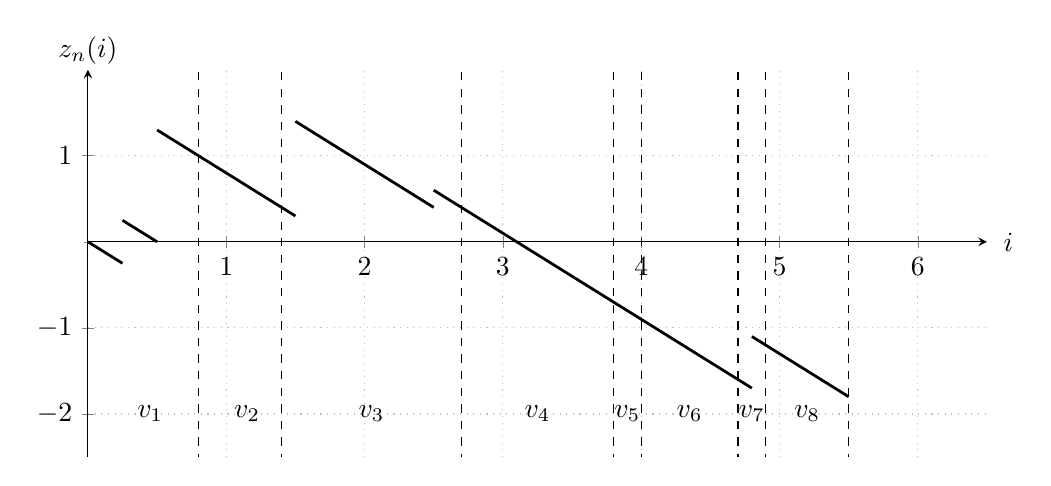
\begin{tikzpicture}

\begin{axis}[
axis x line=bottom,
axis y line=left,
grid = minor,
minor grid style={dotted},
xmin=0,
axis lines = middle,
xmax=6.5,
ymax = 2,
ymin  = -2.5,
xlabel={$i$},
x label style = {at={(axis description cs:1.04,0.555)},anchor=east},
ylabel={$z_n(i)$},
y label style = {at={(axis description cs:0,1.11)},anchor=north},
xtick={1,...,6},
minor xtick = {1,...,6},
ytick={-2,...,1},
minor ytick={-2,...,1},
width = 13cm,
height = 6.5cm
]


% BF WALK LINE
\addplot [line width=1.0pt]coordinates{(0,0) (0.25,-0.25)}; 
% JUMP 0.5
\addplot [line width=1.0pt]coordinates{(0.25,0.25) (0.5,0)}; 
% JUMP 1.3
\addplot [line width=1.0pt]coordinates{(0.5,1.3) (0.9,0.9)};

\addplot [line width=1.0pt]coordinates{(0.9,0.9) (1.5,0.3)}; 
% JUMP 1.1
\addplot [line width=1.0pt]coordinates{(1.5, 1.4) (2.5, 0.4)};
% JUMP 0.2
\addplot [line width=1.0pt]coordinates{(2.5, 0.6) (4.8,-1.7)};
% JUMP 0.6
\addplot [line width=1.0pt]coordinates{(4.8,-1.1) (5.5,-1.8)};

% VERTEX BORDERS
\addplot [dashed] coordinates {(0.8, -7) (0.8, 2)};
\addplot [dashed] coordinates {(1.4, -7) (1.4, 2)};
\addplot [dashed] coordinates {(2.7, -7) (2.7, 2)};
\addplot [dashed] coordinates {(3.8, -7) (3.8, 2)};
\addplot [dashed] coordinates {(4.0, -7) (4.0, 2)};
\addplot [dashed] coordinates {(4.7, -7) (4.7, 2)};
\addplot [dashed] coordinates {(4.9, -7) (4.9, 2)};
\addplot [dashed] coordinates {(5.5, -7) (5.5, 2)};

% VERETX LABELS
\node at (axis cs:0.45,-2) {$v_1$};
\node at (axis cs:1.15,-2) {$v_2$};
\node at (axis cs:2.05,-2) {$v_3$};
\node at (axis cs:3.25,-2) {$v_4$};
\node at (axis cs:3.9,-2) {$v_5$};
\node at (axis cs:4.35,-2) {$v_6$};
\node at (axis cs:4.8,-2) {$v_7$};
\node at (axis cs:5.2,-2) {$v_8$};

\end{axis}

\end{tikzpicture} 